\documentclass[11pt]{article}
\usepackage[a4paper,margin=2.15cm]{geometry}
\usepackage{lmodern}
\usepackage{amsmath,amssymb,amsthm,mathtools}
\usepackage{booktabs}
\usepackage{microtype}
\usepackage[hidelinks]{hyperref}
\usepackage{graphicx}
\graphicspath{{figs/}}
\usepackage{enumitem}
\usepackage{titlesec}
\titlespacing*{\section}{0pt}{1.3ex plus .2ex}{0.7ex}
\titlespacing*{\subsection}{0pt}{1.1ex plus .2ex}{0.5ex}

\theoremstyle{plain}
\newtheorem{theorem}{Theorem}[section]
\newtheorem{lemma}[theorem]{Lemma}
\newtheorem{proposition}[theorem]{Proposition}
\theoremstyle{definition}
\newtheorem{definition}[theorem]{Definition}
\newtheorem{remark}[theorem]{Remark}
\newtheorem{example}[theorem]{Example}

\newcommand{\R}{\mathbb{R}}
\newcommand{\eps}{\varepsilon}
\newcommand{\sgn}{\operatorname{sgn}}
\newcommand{\htop}{h_{\mathrm{top}}}
\setlist{itemsep=2pt,topsep=3pt,leftmargin=1.5em}
\setlength{\abovedisplayskip}{5pt}
\setlength{\belowdisplayskip}{5pt}
\setlength{\abovedisplayshortskip}{3pt}
\setlength{\belowdisplayshortskip}{4pt}

\begin{document}

\begin{center}
  {\Large\bfseries Computing the core entropy of real quadratic polynomials}\\[3pt]
  {\small notes accompanying the code in \texttt{src/CoreEntropy.jl}}
\end{center}
\vspace{2pt}

\section{Introduction}

For $\lambda\in[2,4]$ let
\begin{equation}\label{eq:g}
  g_\lambda(x)=\lambda x(1-x),\qquad x\in[0,1].
\end{equation}
The map $g_\lambda$ is unimodal, with critical point $\tfrac12$: it increases from $0$ to the
critical value $\lambda/4$ on $[0,\tfrac12]$ and decreases back to $0$ on $[\tfrac12,1]$.
Its \emph{core entropy}
$h(\lambda)$ is the topological entropy of $g_\lambda$ restricted to its Hubbard tree, the
smallest invariant interval carrying the critical point and its orbit.  Equivalently ---
and this is how it will be computed --- it is the exponential growth rate of the number of
laps of the iterates $g_\lambda^n$.

As $\lambda$ runs from $2$ to $4$ the parameter crosses the real slice of the quadratic
family and $h$ rises from $0$ to $\log2$, but not smoothly.  It is constant on every
hyperbolic component, that is, on every interval of parameters for which an attracting
cycle (a periodic orbit whose multiplier, the product of $g_\lambda'$ along one turn, has
modulus less than one) exists, and it changes
only on the complement of their union.  The graph is
therefore a devil's staircase, with a plateau for each attracting cycle and a Cantor-like
set of parameters on which the increase takes place.  The continuity of $h$ in $\lambda$ is
a theorem of Milnor and Thurston \cite[Lemma 12.3]{MT}: the growth number of a piecewise
monotone map is continuous in the map at fixed lap number, which is the sense in which the
logistic family moves.  For real parameters Tiozzo \cite{Tiozzo} proved the formula relating
the entropy to the dimensions of sections of the Mandelbrot set, and he later proved
continuity of the core entropy for all quadratic polynomials, as a function of the external
angle, in \cite{Tiozzo2}.

The purpose of this note is to record the algorithm by which the staircase is computed,
the conventions it uses and the control it keeps over the truncation error.
Section~\ref{sec:core} fixes the object, \S\ref{sec:kneading} recalls the kneading theory
that turns the entropy into a root of a power series, \S\ref{sec:model} the piecewise-linear
model, how its semi-conjugacy is computed and when it is a conjugacy, \S\ref{sec:algo}
and~\ref{sec:error} describe
and analyse the numerical scheme, and \S\ref{sec:validation} collects the evidence that the
implementation is correct.  The bands of the limit set, and the renormalization they carry,
are the subject of the companion note \texttt{bands.tex}, which also draws
the corresponding complex picture.  The code,
\texttt{src/CoreEntropy.jl}, follows the same order; the two front ends contain no
mathematics of their own.

\section{The core entropy of a real quadratic polynomial}\label{sec:core}

Everything below is stated for the logistic family, but the object it computes is usually
defined for the quadratic family $f_c(z)=z^2+c$, and the two are the same thing:

\begin{lemma}\label{lem:conj}
Let $\psi_\lambda(x)=\tfrac{\lambda}{2}-\lambda x$.  Then
$\psi_\lambda\circ g_\lambda=f_c\circ\psi_\lambda$, where
\begin{equation}\label{eq:c}
  c=\frac{\lambda}{2}-\frac{\lambda^2}{4}=\frac{\lambda(2-\lambda)}{4}.
\end{equation}
The map $\lambda\mapsto c$ decreases from $c=0$ at $\lambda=2$ to $c=-2$ at $\lambda=4$,
with inverse $\lambda=1+\sqrt{1-4c}$ on this range.
\end{lemma}

\begin{proof}
Substituting $x=\tfrac12-z/\lambda$ gives $x(1-x)=\tfrac14-z^2/\lambda^2$, hence
$\psi_\lambda(g_\lambda(x))=\tfrac{\lambda}{2}-\lambda^2\bigl(\tfrac14-z^2/\lambda^2\bigr)
=\tfrac{\lambda}{2}-\tfrac{\lambda^2}{4}+z^2$.  The derivative of \eqref{eq:c} is
$\tfrac12-\tfrac{\lambda}{2}$, which is negative for $\lambda>1$, so $c$ decreases; the
inverse is the positive root of $\lambda^2-2\lambda+4c=0$.
\end{proof}

Thus $g_\lambda$ on $[0,1]$ is the quadratic family on a real interval, conjugated by an
orientation-reversing affine map, and the parameter range $\lambda\in[2,4]$ corresponds to
$c\in[-2,0]$.

\begin{definition}\label{def:core}
Let $c$ lie in the Mandelbrot set, $K_c$ the filled Julia set of $f_c$ and
$P_c=\overline{\{f_c^n(0):n\ge0\}}$ the postcritical set.  The \emph{Hubbard tree}
$T_c\subset K_c$ is the smallest connected closed set containing $P_c$, and the
\emph{core entropy} is $h(c)=\htop(f_c|_{T_c})$.
\end{definition}

The Hubbard tree is the part of the Julia set that carries the postcritical dynamics: the
Julia set itself may be a complicated fractal, while $T_c$ is a finite tree on which $f_c$
acts as a Markov map (each edge of $T_c$ is mapped over a union of edges).  For real
parameters the tree degenerates to an interval, and
the whole theory becomes one-dimensional.  Indeed, for $c\in[-2,\tfrac14]$ the set $K_c\cap\R$
is an interval, so $T_c=[\min P_c,\max P_c]$ is a real interval; since $f_c$ maps $P_c$ to
itself and is continuous, $f_c(T_c)\subset T_c$.  For $c\in[-2,0]$ the critical point $0$
belongs to $T_c$ and is its only turning point --- a minimum, because $f_c'=2z$ is negative
to the left of $0$ and positive to the right.  Passing back through the orientation
reversing conjugacy of Lemma~\ref{lem:conj}, the core becomes the convex hull of
$\{\tfrac12\}\cup\{g_\lambda^n(\tfrac12)\}$, on which $g_\lambda$ is unimodal with a
\emph{maximum} at $\tfrac12$.  The theory below is formulated for this map; we write
$h(\lambda)=h(c(\lambda))$.

Since the core is the smallest invariant interval, every orbit outside it eventually falls
into it, so the entropy of $g_\lambda$ on all of $[0,1]$ agrees with $h(\lambda)$; for a
unimodal map the entropy is in any case determined by the itinerary of the critical point,
which the core contains.  Four values anchor the computation and serve as tests: $h(2)=0$,
because the critical point is fixed ($c=0$) and the map is conjugate to $z\mapsto z^2$ on
an interval; $h(1+\sqrt5)=0$, the centre of the period-$2$ component, the basilica ($c=-1$),
where the
critical point has period $2$; $h=0$ on the whole period-doubling cascade (the sequence of
period doublings $2,4,8,\dots$) up to the Feigenbaum parameter $\lambda_\infty\approx3.5699457$,
where an attracting cycle always
captures the critical orbit; and $h(4)=\log2$, the Chebyshev case $c=-2$ (the map
$z\mapsto z^2-2$), where $g_4$ is
conjugate to the full tent map.

\begin{figure}
  \centering
  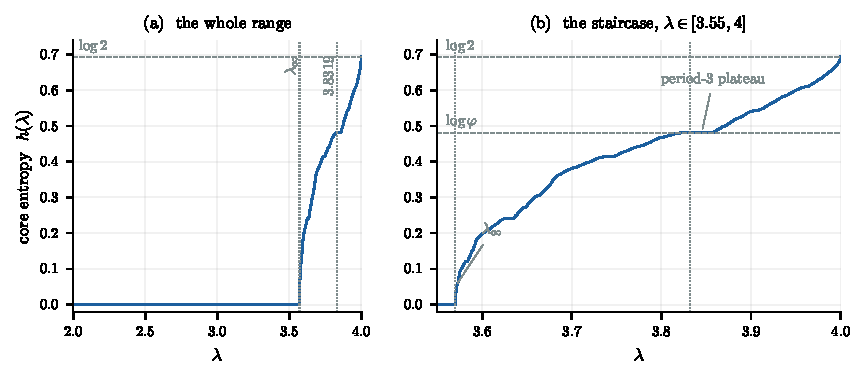
\includegraphics[width=\textwidth]{fig_output}
  \caption{The core entropy of $g_\lambda$ on $[2,4]$, as computed by the code described
  here on $28\,696$ parameters, against the bifurcation diagram of the same parameters (the
  limit set, or attractor, as a greyscale density, read on the right-hand axis, with $x=1$
  at the height of
  $\log2$).  (a)~The whole range: $h$
  vanishes identically up to the Feigenbaum parameter $\lambda_\infty$ and reaches $\log2$
  at $\lambda=4$.  (b)~The staircase on $[3.55,4]$; the horizontal dashed lines are
  $\log\tau$, with $\tau=(1+\sqrt5)/2$, and $\log2$, and the vertical dotted lines mark the
  Feigenbaum parameter
  $\lambda_\infty$ and the period-$3$ centre $3.8319$.}
  \label{fig:output}
\end{figure}

Figure~\ref{fig:output} is the output of the code on $28\,696$ parameters of $[2,4]$.
Panel~(a) is the whole range: $h$ vanishes identically up to the Feigenbaum parameter
$\lambda_\infty$, where the period-doubling cascade accumulates, and then climbs to
$\log2$.  Panel~(b) resolves the climb.  It is not a curve but a staircase --- a flat step
for every hyperbolic component, joined by steep pieces on which the parameter passes
through the complement of the hyperbolic components --- and the widest of the steps is the
one at $\log\tau$, whose
length is explained in \S\ref{sec:validation}.

\section{Kneading theory}\label{sec:kneading}

\subsection{Itineraries, laps and entropy}

The combinatorial type of an orbit is recorded by the sequence of sides of the critical
point it visits.  Since $g_\lambda$ is monotone on each side, this sequence determines
everything that monotonicity can see, and in particular it determines the entropy.

\begin{definition}
For $x\in[0,1]$ the \emph{itinerary} $\iota(x)=(\iota_0(x),\iota_1(x),\dots)$ is given by
$\iota_k(x)=0$ if $g_\lambda^k(x)<\tfrac12$ (left of the critical point),
$\iota_k(x)=1$ if $g_\lambda^k(x)>\tfrac12$ (right), and $\iota_k(x)=*$ if
$g_\lambda^k(x)=\tfrac12$.  A \emph{lap} of a continuous interval map
$F$ is a maximal interval on which $F$ is monotone, and $\ell(F)$ denotes its number of
laps; we write $\ell_n=\ell(g_\lambda^n)$.
\end{definition}

\begin{lemma}\label{lem:laps}
For every $n\ge1$ the laps of $g_\lambda^n$ are exactly the nonempty sets
\[
  I_w=\{x\in[0,1]:\iota_0(x)\cdots\iota_{n-1}(x)=w\},\qquad w\in\{0,1\}^n,
\]
and $g_\lambda^n$ is monotone on each of them.  Hence $\ell_n$ equals the number of
\emph{admissible} words of length $n$, the words that occur as itineraries.
\end{lemma}

\begin{proof}
For $n=1$ this is the definition of the two laps $[0,\tfrac12]$ and $[\tfrac12,1]$.
Suppose the assertion holds for $n$ and let $I_w$ be a lap of $g^n$; on it $g^n$ is
monotone, so $g^{n+1}$ is monotone exactly on the two pieces where $g^n(x)<\tfrac12$ and
$g^n(x)>\tfrac12$, namely $I_{w0}$ and $I_{w1}$.  These are intervals because $g^n$ is
monotone on $I_w$, and every lap of $g^{n+1}$ arises from exactly one lap of $g^n$ in this
way.  A nonempty $I_w$ is maximal, since enlarging it would add points whose itinerary
differs from $w$ in the first $n$ symbols.
\end{proof}

\begin{figure}
  \centering
  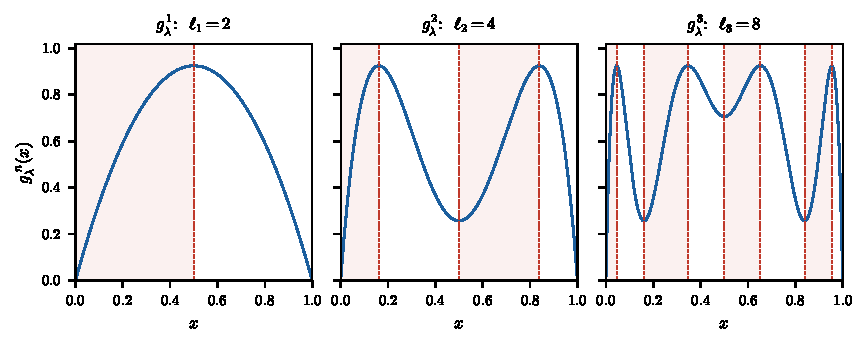
\includegraphics[width=\textwidth]{fig_laps}
  \caption{Laps at $\lambda=3.7$.  (a)~$g_\lambda$, with its two laps shaded alternately and
  the critical point marked by the red dashed line.
  (b)~the sixth iterate $g_\lambda^6$, drawn on a grid of $3000$ points: its $38$ laps are
  the oscillations of the graph.  (c)~the sixth iterate of the tent map of \S\ref{sec:model},
  of slope $e^{h(\lambda)}=1.4648$, which has the same $38$.}
  \label{fig:laps}
\end{figure}

Figure~\ref{fig:laps} illustrates the lemma at $\lambda=3.7$.  Panel~(a) shows $g_\lambda$
with its two laps; panel~(b) the sixth iterate on a fine grid, where the laps are the
oscillations and there are $38$ of them; panel~(c) the sixth iterate of the tent map that
\S\ref{sec:model} associates with the same parameter, which has the same $38$.  The counts
for $n=1,2,4,6,8$ are $2,\,4,\,14,\,38,\,90$.  The first values look like $2^n$, and to
begin with they are, since a lap of $g^n$ has at most two preimage-laps under $g$; the count
falls away from $2^n$ only once the preimage tree is pruned, which happens because a point
$y>\lambda/4$, the maximum of $g_\lambda$, has no real preimage at all.  The growth rate at
$\lambda=3.7$ is $e^{h}=e^{0.3817}\approx1.46$, far below $2$: the interval is not folded
everywhere.

The lemma turns a dynamical quantity into a combinatorial one, and the entropy is the
exponential growth rate of the count:

\begin{theorem}[Misiurewicz--Szlenk \cite{MS}]\label{thm:MS}
For a piecewise monotone interval map (one with finitely many laps),
$\displaystyle h=\lim_{n\to\infty}\frac1n\log\ell_n$.
\end{theorem}

The limit exists because $\ell_{m+n}\le\ell_m\ell_n$ --- cutting a lap of $g^{m+n}$ by
$g^m$ gives at most $\ell_m$ pieces, each monotone for $g^n$ --- so $\log\ell_n$ is
subadditive and the limit equals the infimum.  Since $g_\lambda$ has two laps, $\ell_n\le2^n$
and therefore
\begin{equation}\label{eq:bound}
  0\le h(\lambda)\le\log2 .
\end{equation}

For the entropy one only needs the growth rate, but $\ell_n$ itself grows like $e^{hn}$, so
enumerating laps is exponentially expensive and useless beyond small $n$.  The kneading
determinant computes the growth rate from a single sequence of signs.

\subsection{The kneading sequence and the determinant}

\begin{definition}\label{def:kneading}
Let $x_k=g_\lambda^k(\tfrac12)$.  The \emph{kneading sequence} $\nu=\nu_1\nu_2\cdots$ is
the itinerary of the critical value: $\nu_k$ is the symbol of $x_k$.  If $x_k=\tfrac12$ for
some $k\ge1$, that is, if the critical point is periodic of period $k$, then $\nu_k=*$ and
the sequence is declared periodic of period $k$, with $*$ read as $1$ in all later
positions.
\end{definition}

The sequence $\nu$ is the complete combinatorial invariant of the critical orbit, and by
the results of \cite{MT} it determines the entropy.  When the critical point is periodic
the itinerary is undefined at the return, and the symbol has to be given a value.  We read
$*$ as $1$, so that $s_k=-1$ there.

\begin{definition}\label{def:eps}
The \emph{sign sequence} is $s_k=\sgn g_\lambda'(x_k)$.  Since
$g_\lambda'=\lambda(1-2x)$, one has $s_k=+1$ when $x_k<\tfrac12$ and $s_k=-1$ when
$x_k>\tfrac12$; at a critical hit $x_k=\tfrac12$ we set $s_k=-1$, which is exactly the
rule ``read $*$ as $1$'', the symbol of the decreasing branch.  With $\eps_0=1$ put
\begin{equation}\label{eq:eps}
  \eps_k=s_1s_2\cdots s_k\qquad(k\ge1).
\end{equation}
\end{definition}

The sign $s_k$ records which branch of $g_\lambda$ the orbit is on at time $k$, and the
product $\eps_k$ records the orientation of $g_\lambda^k$ on the lap whose itinerary is the
first $k$ symbols of $\nu$: the map is increasing there when $\eps_k=+1$ and decreasing
when $\eps_k=-1$.

The value given to $*$ does not affect the entropy.  Suppose $\nu$ has period $k$, and let
$\eps$ and $\eps'$ be the sign sequences of the two fillings.  They differ only in the
$k$-th symbol of each period, so $\eps'_j=(-1)^{\lfloor j/k\rfloor}\eps_j$: one filling has
$\eps$ of period $k$ and the other of period $2k$, since $s_k$ changes sign and with it
$\prod_{r\le k}s_r$.  With $P(t)=\sum_{r<k}\eps_rt^r$, the same for both, the two
determinants are
\begin{equation}\label{eq:fillings}
  D(t)=\frac{P(t)}{1-t^k},\qquad D'(t)=\frac{P(t)}{1+t^k},
\end{equation}
in some order.  Neither denominator vanishes on $(0,1)$, so there $D$ and $D'$ vanish
exactly at the zeros of the common numerator $P$: they have the same smallest zero $t_0$ and
the same entropy.  The factor $(1-t^k)/(1+t^k)$ is the one by which Milnor and Thurston
extend their continuity lemma to a map with a periodic turning point \cite[Lemma 12.3]{MT}.
At the period-$3$ centre, for instance, $P=1-t-t^2$ and $t_0=1/\tau$ whichever filling is
used.

The two fillings are also literally the two codes seen on the two sides of the parameter.  A
return is transversal: with $x_k(\lambda)=g_\lambda^k(\tfrac12)$ and
$x_k(\lambda_0)=\tfrac12$ one has
$x_k(\lambda_0+\epsilon)-\tfrac12=a_k\epsilon+O(\epsilon^2)$, where
$a_k=\frac{d}{d\lambda}x_k(\lambda_0)\neq0$.  So the orbit passes on one side of the critical
point below $\lambda_0$ and on the other side above it, and instead of closing it is
attracted to the nearby $k$-cycle.  The cycle point nearest $\tfrac12$ agrees with $x_k$ to
first order, differing from it by $\tfrac12(g^k)''(\tfrac12)a_k^2\epsilon^2$ because $g^k$ is
critical at $\tfrac12$; the itinerary is therefore exactly $k$-periodic, with no transient,
and the sign of $a_k$ decides which filling belongs to which side.  At the period-$3$ centre
$a_3=-2.0876\ldots$, and the code is $(1,0,1)$ below $\lambda_3$ and $(1,0,0)$ above it.

\begin{definition}\label{def:D}
The \emph{kneading determinant} of $\nu$ is the power series
\begin{equation}\label{eq:D}
  D(t)=\sum_{k\ge0}\eps_k t^k .
\end{equation}
Since $|\eps_k|=1$ for every $k$, $D$ converges absolutely on the disc $|t|<1$, is
continuous there, and $D(0)=1$.
\end{definition}

\begin{figure}[t]
  \centering
  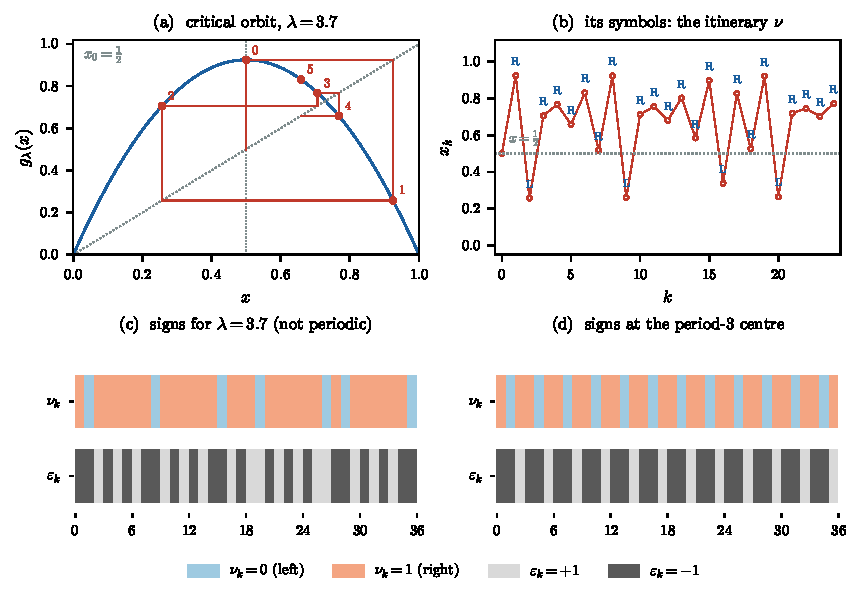
\includegraphics[width=0.94\textwidth]{fig_kneading}
  \caption{The kneading data.  (a)--(c)~at $\lambda=3.7$: the cobweb of the critical
  orbit, with the dotted diagonal $y=x$ and the dotted level $\tfrac12$; the same orbit
  against time with the symbol of each point written above it; and
  the itinerary $\nu$ together with the partial products $\eps_k$.  (d)~at the period-3
  centre $\lambda=3.8319$, where the critical point returns to $\tfrac12$ and both
  sequences are periodic: $(1,0,*)$ repeated, with $*$ read as~$1$.  In panel~(b) the
  letters are the symbols: L is $0$, R is $1$.}
  \label{fig:kneading}
\end{figure}

Figure~\ref{fig:kneading} shows what the data look like for one parameter.  Panel~(a) is
the cobweb of the critical orbit on the graph of $g_\lambda$: from $x_0=\tfrac12$ the orbit
jumps to the critical value and then wanders.  Panel~(b) plots the same numbers against
time and records above each point the symbol of the side it lies on; that string is the
itinerary $\nu$.  Panel~(c) displays it as a strip of cells together with the partial
products $\eps_k$.  Each is a sequence of signs and nothing more, and the content of
\S\ref{sec:kneading} is that these signs determine the entropy.  Panel~(d) repeats the
exercise at the period-3 centre, where the critical point returns to $\tfrac12$ after three
steps: the string is then periodic, $(1,0,*)$ repeated with $*$ read as $1$, and this
periodicity of the data is exactly what makes the determinant rational in
\S\ref{sec:pcf}.

\subsection{The zero of the determinant is the growth rate}

\begin{theorem}[Milnor--Thurston \cite{MT}; see also \cite{dMvS}, Ch.~II]\label{thm:MT}
Let $h$ be the topological entropy of $g_\lambda$.  If $h>0$ then $D(e^{-h})=0$ and
$D(t)>0$ for $0<t<e^{-h}$.  If $h=0$ then $D(t)>0$ for all $t\in(0,1)$.
\end{theorem}

Consequently $e^{-h}$ is the smallest zero of $D$ in $(0,1)$, and
\begin{equation}\label{eq:h}
  h(\lambda)=\log\frac{1}{t_0},\qquad t_0=\min\{t\in(0,1):D(t)=0\},
\end{equation}
with the convention that no such $t_0$ exists exactly when $h=0$.  By \eqref{eq:bound},
$t_0\ge\tfrac12$ whenever $h>0$.  This is the identity on which the whole computation
rests: it replaces a limit of lap counts by the root of a series with coefficients
$\pm1$.  Figure~\ref{fig:determinant}(a) shows such a zero.

\begin{remark}[why a zero of $D$ is a growth rate]
The reciprocal $1/D$ is the kneading zeta function of the map: its coefficients count
periodic orbits with signs determined by their itineraries \cite{MT}.  For a piecewise
monotone map the number of periodic orbits grows like $e^{hn}$, so $1/D$ has radius of
convergence $e^{-h}$.  By Pringsheim's theorem a series with nonnegative
coefficients is singular on the positive axis; here $1/D$ is singular at $t=e^{-h}$, so $D$
vanishes there.  The second half
of the theorem, the absence of zeros below $e^{-h}$, says that this is the \emph{first}
singularity and is what makes the smallest zero the correct one to take.  We use the
theorem as a black box and test it in \S\ref{sec:validation}.
\end{remark}

\subsection{The postcritically finite case, exactly}\label{sec:pcf}

A map is \emph{postcritically finite} when its critical orbit is finite; here we treat the
case in which it is periodic, which makes the determinant rational.  In the quadratic family
a parameter at which the critical point is strictly preperiodic --- the critical orbit finite
but not periodic --- is called a \emph{Misiurewicz point}.  When the critical orbit
is periodic of period $k$ the sign sequence is $k$-periodic, so
$\eps$ is periodic with period $k$ or $2k$ and $D$ is a rational function
$D=P(t)/(1-t^{p})$ whose numerator $P$ has degree $p-1$ and integer coefficients.  The
zeros of $D$ are then the zeros of $P$, and $t_0$ is the smallest of them in
$(0,\tfrac12)$: an algebraic number that can be computed exactly, with no truncation at
all.  Three such parameters serve as tests.

\begin{example}[$\lambda=4$, the Chebyshev case]\label{ex:lambda4}
Here $x_1=1$ and $x_k=0$ for $k\ge2$, so $s=(-1,+1,+1,\dots)$ and $\eps_k=-1$ for every
$k\ge1$.  Summing the geometric tail,
\[
  D(t)=1-\frac{t}{1-t}=\frac{1-2t}{1-t},
\]
whose smallest positive zero is $t_0=\tfrac12$; hence $h=\log2$, as it must be for a map
conjugate to the tent map.
\end{example}

\begin{example}[$\lambda=1+\sqrt5$, the basilica]\label{ex:basilica}
The critical orbit is $\tfrac12\mapsto\tfrac{\lambda}{4}\mapsto\tfrac12$, so $\nu=1*$ and
every $s_k=-1$.  Then $D(t)=\frac{1}{1+t}$, which has no zero in $(0,1)$, and the theorem
correctly reports $h=0$: the critical orbit is attracted to a $2$-cycle and the core
supports no exponential complexity.
\end{example}

\begin{example}[the period-3 centre]\label{ex:p3}
Let $c_3$ be the real root of $c^3+2c^2+c+1=0$ (so $c_3=-1.7548776662\ldots$), the centre
of the period-$3$ component, and $\lambda_3=1+\sqrt{1-4c_3}$.  The critical orbit has
period $3$ with itinerary $(1,0,*)$,
so $s=(-1,+1,-1)$ repeated and $\eps$ has period $3$ with $\eps=(1,-1,-1)$.  Hence
\[
  D(t)=\frac{1-t-t^2}{1-t^3},
\]
whose smallest zero in $(0,1)$ is $t_0=1/\tau$ with $\tau=\tfrac{1+\sqrt5}{2}$, so
$h(\lambda_3)=\log\tau=0.481211825\ldots$.
\end{example}

In both cases the entropy is settled by a polynomial rather than a series: the determinant
is rational and its smallest zero can be read off exactly, with no truncation at all.

\section{The piecewise-linear model}\label{sec:model}

The lap counts of \S\ref{sec:kneading} are not special to the quadratic family: every
piecewise monotone map with growth number $s=e^{h}>1$ --- the exponential growth rate of its
lap numbers --- is topologically semi-conjugate to a piecewise linear map of slope $\pm s$,
that is, there is a continuous nondecreasing surjection intertwining the two maps.  For the
logistic family that model is the tent map of
slope $s=e^{h(\lambda)}=1/t_{0}$.  This section states the theorem and then explains how the
semi-conjugacy is actually computed --- a computation the entropy does not need, but which
shows that the two lap counts agree, and which is a good deal simpler than the trees of
\S\ref{sec:kneading} might suggest.

\subsection{The theorem}

\begin{theorem}[Milnor--Thurston \cite{MT}, Theorem 7.4, in the notation of this paper]\label{thm:model}
Suppose $h(\lambda)>0$ and put $s=e^{h(\lambda)}=1/t_0$.  Then there is a continuous
nondecreasing surjection $A:[0,1]\to[0,1]$ such that
\[
  f_s\bigl(A(x)\bigr)=A\bigl(g_\lambda(x)\bigr)\qquad\text{for every } x\in[0,1],
\]
where $f_s(y)=sy$ for $y\le\tfrac12$ and $f_s(y)=s(1-y)$ for $y\ge\tfrac12$.
\end{theorem}

The map supplied by \cite[Theorem 7.4]{MT} is piecewise linear with slope $\pm s$; since
$g_\lambda$ has two laps the model has at most two, and since $s>1$ it cannot have fewer, so
it is $f_s$.  That is the only point of the quoted statement that has to be checked to read
it in the notation used here.

The map $A$ is not always a conjugacy (an invertible semi-conjugacy): it may collapse
intervals to points, and in particular
the basin (the set of points whose orbits converge to it) of an attracting cycle of
$g_\lambda$ goes to a cycle of $f_s$
(\S\ref{sec:conjugacy}).  The arrow does not reverse --- a tent map has no attracting cycle,
while $g_\lambda$ may have one.  What it buys
the computation is a second view of the lap numbers: since $f_s(A(x))=A(g_\lambda(x))$, the
map $A$ carries every lap of $g_\lambda^n$ into a lap of $f_s^n$, so
$\ell(f_s^n)\le\ell(g_\lambda^n)$, and both grow like $s^n$.  At $\lambda=3.7$ they agree at
every $n$ we computed, as panels~(b) and~(c) of Figure~\ref{fig:laps} show for $n=6$.

\subsection{Computing the semi-conjugacy}\label{sec:computingA}

The functional equation determines $A$, and also computes it.  Since $A$ is monotone and
$f_s$ increases on $[0,\tfrac12]$ and decreases on $[\tfrac12,1]$, the side of $x$ decides
which branch of $f_s$ to invert:
\begin{equation}\label{eq:Abranch}
  A(x)=
  \begin{cases}
    A\bigl(g_\lambda(x)\bigr)/s, & x<\tfrac12,\\[2pt]
    1-A\bigl(g_\lambda(x)\bigr)/s, & x>\tfrac12 .
  \end{cases}
\end{equation}
Write $T_0(u)=u/s$ and $T_1(u)=1-u/s$ for the two inverse branches, and $w_0w_1\cdots$ for
the itinerary of $x$, so that $w_k$ records the side on which $g_\lambda^k(x)$ lies.
Iterating \eqref{eq:Abranch} gives
\begin{equation}\label{eq:A}
  A(x)=T_{w_0}\circ T_{w_1}\circ\cdots\circ T_{w_{n-1}}\bigl(A(g_\lambda^n x)\bigr).
\end{equation}
Both branches have slope $1/s$, so the composition is a contraction of ratio $s^{-n}$ and the
seed $A(g_\lambda^n x)\in[0,1]$ matters less than $s^{-n}$:
\begin{equation}\label{eq:Alim}
  A(x)=\lim_{n\to\infty}T_{w_0}\circ\cdots\circ T_{w_{n-1}}(u),
\end{equation}
for any $u\in[0,1]$, the error after $n$ steps being at most $s^{-n}$.

That is the algorithm: iterate $g_\lambda$ from $x$ recording the symbols, then push any seed
through the corresponding affine maps in reverse order.  It costs $O(n)$ per point and never
touches the preimage tree, which is what makes it robust where the obvious alternative fails.
Pairing the turning points of $g_\lambda^n$ with those of $f_s^n$ --- that is, matching the
two trees level by level --- only works while the trees have the same size, and at
$\lambda=3.84$ they do not: the critical point of $f_s$ is there periodic of period $3$,
while the critical orbit of $g_\lambda$ merely approaches a cycle, so a whole branch of the
logistic tree is collapsed by $A$ and the counts differ already at level three.

Two remarks on accuracy.  A symbol misread at step $k$ perturbs the result by at most
$s^{-k}$, the diameter of the image after $k$ steps, so only the early symbols matter --- and
those are exactly the ones a double-precision orbit gets right (\S\ref{sec:float}).  The
seed error is $s^{-n}$: at $\lambda=3.7$, where $s=1.4648$, $n=64$ gives
$2.5\times10^{-11}$, while near $\lambda=4$ the same $n$ gives $5\times10^{-20}$.  The
implementation takes $n=64$ and checks itself against the functional equation, evaluating
$\max_x|f_s(A(x))-A(g_\lambda(x))|$ on the $241$ points $x=i/240$; at
$\lambda=3.7,\,3.84,\,3.86,\,4$ that maximum is $5.7\times10^{-12}$, $1.3\times10^{-14}$,
$1.0\times10^{-14}$ and $2.2\times10^{-16}$.

\begin{figure}
  \centering
  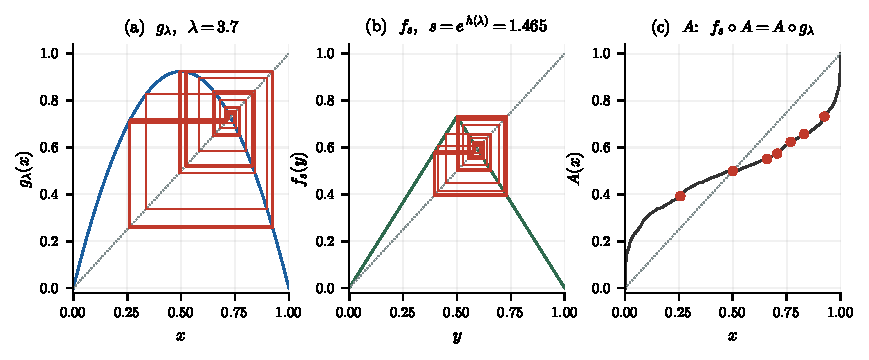
\includegraphics[width=0.95\textwidth]{fig_model}
  \caption{The three objects at $\lambda=3.7$.  (a)~$g_\lambda$, with the cobweb of the
  critical orbit.  (b)~the tent map $f_s$ of slope $s=e^{h(\lambda)}=1.4648$, with its own
  cobweb.  (c)~the map $A$ of Theorem~\ref{thm:model}, on which the iterates of the critical
  orbit of $f_s$ (abscissae) sit at the corresponding iterates of $g_\lambda$ (ordinates).
  The dotted diagonal is $y=x$ in all three panels.}
  \label{fig:model}
\end{figure}

\subsection{When the semi-conjugacy is a conjugacy}\label{sec:conjugacy}

Since $A$ is monotone, it fails to be injective exactly when it collapses a nondegenerate
interval to a point.  Here $\Lambda$ is Milnor and Thurston's growth measure
\cite[\S7]{MT}: $\Lambda(J)$ is the asymptotic fraction of laps of $g_\lambda^n$ that lie in
$J$, so $\Lambda$ is finitely additive and $\Lambda(g_\lambda(J))=s\Lambda(J)$ whenever
$g_\lambda|J$ is a homeomorphism.  Collapses propagate: if $A$ collapses $J$, so that
$\Lambda(J)=0$, then
$\Lambda(g_\lambda^n(J))=0$ for every $n\ge0$, because $g_\lambda^n(J)$ is a union of intervals
on which $g_\lambda^n$ is monotone, each of which is collapsed by Lemma~7.3 of \cite{MT}.  The
question is therefore which intervals can be collapsed.

An interval $J$ is a \emph{homterval} if every iterate $g_\lambda^n$ is monotone on it,
equivalently if no iterate carries a point of $J$ to the critical point $\tfrac12$.  All points
of a homterval have the same itinerary, so $A$ is constant on it.  For the quadratic family the
homtervals are exactly the intervals in the basins of the attracting and neutral (parabolic)
cycles: a
homterval is either attracted to such a cycle or wandering (its images are pairwise disjoint),
and an $S$-unimodal map (one with negative Schwarzian and a non-flat critical point) has no
wandering intervals \cite{dMvS,Guck}.  For an attracting cycle this is Singer's theorem: the
critical point lies in its basin \cite{Sing}, and a parabolic (neutral) cycle attracts it as
well.  So an attracting or a parabolic cycle makes $A$ strict, and if there is no such
cycle the itinerary map of $g_\lambda$ is injective.

That is not the end of the story, because $f_s$ has a critical point too, and the two inverse
branches of \eqref{eq:Alim} agree there:
\[
  T_0(s/2)=T_1(s/2)=\tfrac12 .
\]
If $f_s^k(\tfrac12)=f_s^j(\tfrac12)$ for some $k>j\ge0$, then for every $x$
\begin{equation}\label{eq:ident}
  A\bigl(g_\lambda^k(x)\bigr)=f_s^k\bigl(A(x)\bigr)
  =f_s^j\bigl(A(x)\bigr)=A\bigl(g_\lambda^j(x)\bigr),
\end{equation}
and if $g_\lambda^k(x)\ne g_\lambda^j(x)$, monotonicity makes $A$ constant on the interval
between them.  At $x=\tfrac12$ this is a genuine collapse unless the critical orbit of
$g_\lambda$ has the same coincidence.  The critical orbit of $f_s$ is eventually periodic for a
countable set of slopes, namely the growth numbers of the periodic and preperiodic
(eventually periodic) kneading
sequences; on the corresponding level sets of $h$ the collapse \eqref{eq:ident} therefore takes
place unless $g_\lambda$'s critical orbit is preperiodic with exactly the same pattern.

\begin{proposition}\label{prop:conj}
For $s=e^{h(\lambda)}>1$ the following are equivalent:
\begin{enumerate}[label=(\roman*)]
  \item $A$ is injective;
  \item $g_\lambda$ is topologically conjugate to $f_s$;
  \item $g_\lambda$ has no homterval, and $g_\lambda^k(\tfrac12)=g_\lambda^j(\tfrac12)$ for
        every $k>j\ge0$ with $f_s^k(\tfrac12)=f_s^j(\tfrac12)$.
\end{enumerate}
\end{proposition}

\begin{proof}
(i)$\Leftrightarrow$(ii): a monotone surjection is a homeomorphism exactly when it is
injective, and $f_s(A(x))=A(g_\lambda(x))$ then exhibits the conjugacy.  (ii)$\Rightarrow$(iii):
a conjugacy carries homtervals to homtervals and the critical orbit of $g_\lambda$ to that of
$f_s$, and $f_s$ has no homterval because $|f_s'|=s>1$ wherever it is differentiable.
(iii)$\Rightarrow$(i): if $A(x)=A(y)$ for $x<y$, then either the two points have equal
itineraries --- and then $[x,y]$ is a homterval --- or some iterate maps $[x,y]$ across the
critical point; in the second case the two itineraries are exchanged by the two inverse
branches at the critical value of $f_s$, and following the critical orbit produces a
coincidence $f_s^k(\tfrac12)=f_s^j(\tfrac12)$ with $g_\lambda^k(\tfrac12)\ne
g_\lambda^j(\tfrac12)$.  Both alternatives contradict (iii).
\end{proof}

\begin{table}[htbp]
  \centering\small
  \begin{tabular}{@{}llll@{}}
    \toprule
    $\lambda$ & $h(\lambda)$ & behaviour of $g_\lambda$ & $A$ \\
    \midrule
    $4$ & $\log2$ & $c\mapsto1\mapsto0\mapsto0$ & conjugacy \\
    $3.6785735\ldots$ & $\log\sqrt2$ & $c\mapsto$ repelling fixed point & conjugacy \\
    $3.84$ & $\log\tau$ & attracting $3$-cycle & collapses its basin \\
    $3.85$ & $\log\tau$ & chaotic, $g^3(c)=0.4605$ & collapses $[0.45,0.55]$ \\
    \bottomrule
  \end{tabular}
  \caption{Four parameters illustrating Proposition~\ref{prop:conj}.  The first two are
  conjugacies, the last two are not: at $\lambda=3.84$ the obstruction is the attracting
  cycle, at $\lambda=3.85$ it is the coincidence $f_\tau^3(\tfrac12)=\tfrac12$ in the
  model while $g_\lambda^3(\tfrac12)\ne\tfrac12$.}
  \label{tab:conj}
\end{table}

Table~\ref{tab:conj} collects the examples.  At $\lambda=4$ the semi-conjugacy is
$A(x)=\tfrac2\pi\arcsin\sqrt x$, a homeomorphism.  At
$\lambda=3.6785735104\ldots$ --- the real root of $\lambda^3-2\lambda^2-4\lambda-8=0$, a
Misiurewicz point, where the critical point is strictly preperiodic ---
the critical orbit is
\[
  \tfrac12\longmapsto0.9196433776\longmapsto0.2718445063\longmapsto0.7281554937,
\]
with $0.7281554937$ a repelling fixed point, while the critical orbit of $f_{\sqrt2}$ is
$\tfrac12\mapsto\tfrac{\sqrt2}{2}\mapsto\sqrt2-1\mapsto2-\sqrt2$ and lands on its own fixed point;
the two patterns agree, there is no homterval, and $A$ is a conjugacy.  At $\lambda=3.85$ the
plateau of $A$ has width $0.10$, against $0.08$ at $\lambda=3.84$: on $[0.45,0.55]$ the lap
number of $g_\lambda^n$ is $37$ at $n=16$, while $\tau^{16}\approx2207$, so the interval is
genuinely collapsed.

So ``no attracting cycle'' is not the same as ``$A$ is a conjugacy''.  The extra obstructions
come from the critical orbit of the model, and they occur on the level sets of $h$ that meet
the growth numbers of periodic and preperiodic kneading sequences; the $h=\log\tau$
plateau is the first and largest of them.

\begin{remark}[Uniqueness]\label{rem:unique}
For a unimodal map the semi-conjugacy of Theorem~\ref{thm:model} is unique: any such $A$
carries the turning point to $\tfrac12$, hence preserves itineraries, and $f_s$ has no
homterval, so its itinerary map is injective and $A(x)$ is the unique point of $[0,1]$ with
the itinerary of $x$.  The non-uniqueness of \cite[\S7.8]{MT} therefore needs at least three
laps: the alternative semiconjugacies $A_k$ of \cite[\S7.8]{MT} use one of the $\ell-1$
columns of the inverse kneading matrix, where $\ell$ is the number of laps of the map, and a
unimodal map has only one.
\end{remark}

\section{The algorithm}\label{sec:algo}

The program takes a parameter $\lambda\in[2,4]$ and returns $h(\lambda)$ by locating the
smallest zero of the truncated determinant.  Three constants govern the truncation: the
initial order $N_0=800$, the maximal order $N_{\max}=51200$, and the tolerance $\rho=25$
whose role is explained in \S\ref{sec:error}.  For an order $N$ the series \eqref{eq:D} is
truncated to
$D_N(t)=\sum_{k\le N}\eps_k t^k$.

\paragraph{Step 1: the orbit and its signs.}
Starting from $x=\tfrac12$, for $k=1,\dots,N$ one computes
\[
  x\longleftarrow\lambda x(1-x),\qquad
  s_k\longleftarrow\begin{cases}+1,&x<\tfrac12,\\ -1,&x\ge\tfrac12,\end{cases}
  \qquad\eps_k\longleftarrow\eps_{k-1}s_k .
\]
The comparison is the sign of $g_\lambda'(x_k)$, and the rule $s_k=-1$ at $x=\tfrac12$
implements Definition~\ref{def:kneading}.  The rule is self-consistent: if $x_k=\tfrac12$
then $x_{k+1}=\lambda/4=x_1$, so the orbit repeats from the beginning and the computed sign
sequence is periodic from that point on, exactly as the convention requires.

\paragraph{Step 2: evaluation.}
The truncated determinant is evaluated by Horner's rule,
\[
  D_N(t)=\eps_0+t\bigl(\eps_1+t(\eps_2+\cdots+t\eps_N)\cdots\bigr),
\]
which costs $N$ multiplications and additions, in one pass over the $\eps_k$ and without
forming the powers $t^k$ separately.

\paragraph{Step 3: the smallest zero.}
$D_N$ is continuous on $[0,1]$ with $D_N(0)=1$, and by \eqref{eq:bound} the zero of
interest lies in $[\tfrac12,1]$; the search is confined to $[0.45,\,t_{\max}]$ with
$t_{\max}=1-\rho/N$, the lower end for safety and the upper end because the truncation is
unreliable as $t\to1$ (\S\ref{sec:error}).  A bracket is found in one of two ways.  If the
previous parameter had a zero $t_{\mathrm{prev}}$, one tries
$[t_{\mathrm{prev}}-\delta,t_{\mathrm{prev}}+\delta]$ with $\delta=10^{-4}$, multiplying
$\delta$ by $4$ (up to fourteen times) until $D_N>0$ at the left end and $D_N<0$ at the
right end; since the zero moves continuously with the parameter, this almost always
succeeds and costs a handful of evaluations.  If it fails, $80$ equally spaced points of
$[0.45,t_{\max}]$ are evaluated and the first sign change from $+$ to $-$ is taken.  The
bracket is then refined by bisection until the interval stops shrinking at machine
precision.

\paragraph{Step 4: acceptance, doubling, and the case of zero entropy.}
With $t_0$ in hand, $h=-\log t_0$.  The zero is accepted if $hN\ge\rho=25$ and $N$ is
doubled otherwise, up to $N_{\max}$; if no sign change exists at all, $h$ is reported as
$0$ after one precautionary increase of $N$, from $800$ to $3200$.  Both rules exist to
keep the truncation error under control, and both are justified in \S\ref{sec:error}.

It may help to follow one parameter through the four steps.  For $\lambda=3.7$ the
critical orbit begins $0.5,\,0.925,\,0.2567,\,0.7061,\dots$; its signs are those of
Figure~\ref{fig:kneading}(b) and its partial products those of panel~(c).  With $N=800$
the search runs over $[0.45,0.9688]$, the first sign change is at $t_0=0.6827$, and
$h=-\log t_0=0.38172$ --- the value listed for this parameter in the data set.

A Horner evaluation costs $O(N)$ and a parameter needs of order fifteen of them once the
bracket is inherited, so the sweep of $28\,696$ parameters used for the published data
takes about $1.5$\,s on a single core, the largest order reached being $N=3200$.

\section{Error control}\label{sec:error}

\subsection{Truncation}

Because $|\eps_k|=1$ for every $k$, the tail of \eqref{eq:D} is dominated by a geometric
series, with no information about the orbit beyond the coefficients:
\begin{equation}\label{eq:tail}
  \bigl|D(t)-D_N(t)\bigr|\le\sum_{k>N}t^k=\frac{t^{N+1}}{1-t},\qquad 0<t<1 .
\end{equation}
Write $t_0^{(N)}$ for the smallest zero of $D_N$ and $h_N=-\log t_0^{(N)}$ for the entropy
read off from it; the truncation error in the entropy is $|h_N-h|$.
\begin{figure}
  \centering
  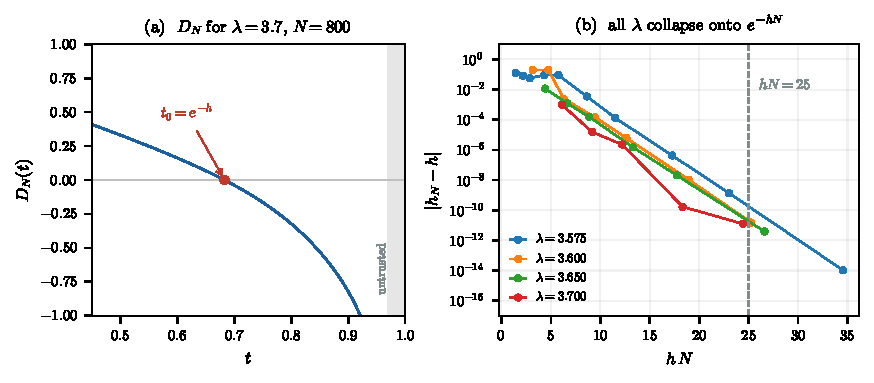
\includegraphics[width=\textwidth]{fig_determinant}
  \caption{The zero and the truncation error.  (a)~$D_N(t)$ for $\lambda=3.7$ and
  $N=800$; its smallest zero is $t_0=e^{-h}$, the grey horizontal line is $D=0$, and
  beyond $t=1-\rho/N$ (shaded) the truncation is no longer controlled.  (b)~$|h_N-h|$
  against $hN$ for four parameters:
  the curves collapse, which is the empirical content of \eqref{eq:tail}; the dashed line
  is the acceptance threshold $hN=25$.}
  \label{fig:determinant}
\end{figure}

This is the only a priori error in the method, and the thresholds of \S\ref{sec:algo} are
chosen to control it.

Figure~\ref{fig:determinant} tests both halves of the analysis.  Panel~(a) shows $D_N$ for
$\lambda=3.7$ with its zero marked, and shades the region $t>1-\rho/N$ in which nothing is
trusted.  Panel~(b) plots the distance between $h_N$ and its limit against $hN$ for four
parameters.  The four curves collapse onto one: the error is governed by
$t_0^{N}=e^{-hN}$ and by nothing else.  The dashed line at $hN=25$ is the acceptance
threshold: by then the error has fallen to about $10^{-10}$, and a few more units of $hN$
would only push it into the roundoff floor.  That is why the value $25$ was chosen rather
than, say, $10$ or $100$.  It is worth stressing that \eqref{eq:tail} holds whatever the
computed signs are, so it also covers the case in which the orbit itself is inaccurate
(see \S\ref{sec:float}).

\subsection{The acceptance criterion}

Let $t_0=e^{-h}$ be the zero of $D$ and suppose $hN\ge\rho$.  Since $1-e^{-h}\ge h/2$ for
$0<h\le1$, the error of the truncated determinant at the true zero is at most
\[
  \bigl|D_N(t_0)\bigr|=\bigl|D(t_0)-D_N(t_0)\bigr|
  \le\frac{e^{-h(N+1)}}{1-e^{-h}}\le\frac{2e^{-25}}{h},
\]
which is at most $3\cdot10^{-9}$ when $h\ge10^{-2}$, and far smaller for larger $h$.  If
$D'(t_0)\ne0$, the zero of $D_N$ differs from $t_0$ by at most this quantity divided by
$|D'(t_0)|$.  The code does not estimate $D'$, so what is rigorously controlled is $D$
rather than $h$ itself.  Where $|D'|$ is of order one that is the end of the matter and the
exact tests of \S\ref{sec:validation} show errors at the level of roundoff.  Near the foot of
the staircase, where $h$ is small but not zero, $|D'|$ is small as well: at
$\lambda=3.57063$, with $h=0.0323$, the computed derivative at the truncated zero is
$D'(t_0)=-1.2\cdot10^{-3}$, so that the bound degrades to $7\cdot10^{-7}$; the residual of
$6\cdot10^{-12}$ which the truncation actually leaves in $D$ there costs $5\cdot10^{-9}$ of
$h$.  Rerunning the sweep with $hN\ge40$ finds that scale: apart from the parameters reported
as zero at the resolution floor, no value moves by more than $5.3\cdot10^{-9}$.

\subsection{The resolution floor}

If there is no sign change in $[0.45,1-\rho/N]$, then either $h=0$ or $0<h<\rho/N$, and the
two alternatives cannot be separated at order $N$.  After raising $N$ to $3200$ the code
reports $0$, so a zero entropy is certified only down to $25/3200\approx0.008$.  The effect
on the data is confined to the foot of the staircase: of the $28\,696$ parameters, exactly
one ($\lambda=3.5699733$, a few $10^{-5}$ above $\lambda_\infty$) is reported as $0$ while
its entropy is $0.0075$.  Recomputing the whole sweep with $N_0=6400$ changes no other
value by more than $10^{-8}$, the residue of the small derivative above, so the floor is much
the largest of the two limitations of the default settings.

\subsection{The floating-point orbit}\label{sec:float}

The signs are read off a double-precision orbit, whose error grows like $e^{\chi k}$
with $\chi$ the Lyapunov exponent, so the itinerary is reliable only up to
$k\approx16\log10/\chi$.  Two mechanisms keep this harmless.  On a hyperbolic component
the critical orbit converges to the attracting cycle and, in floating point, reaches it
exactly after finitely many steps; the computed sign sequence is then the true itinerary
forever, and this covers every plateau of $h$.  And when $h$ is small the parameter is
close to a parabolic or Feigenbaum value, $\chi$ is small, the horizon is far, and the
criterion $hN\ge\rho$ asks for precisely the large $N$ that this accuracy permits.  Beyond
the horizon the tail bound \eqref{eq:tail} makes the unknown terms harmless, since their
total weight is at most $t^N/(1-t)$.

\subsection{Degenerate zeros}

The scan looks for a change of sign, so a smallest zero of even order would be passed over
and a larger value of $h$ reported.  No such case occurred in any test, and in the
postcritically finite case $D$ is a rational function whose zeros are generically simple.
This is the one structural assumption of the search; it is recorded for completeness.

\section{Validation}\label{sec:validation}

\subsection{Parameters with known entropy}

Table~\ref{tab:exact} compares the output with the exact values derived in
\S\ref{sec:kneading}.  The first three are the cases of vanishing entropy, in which
the second assertion of Theorem~\ref{thm:MT} applies; the last two are
Examples~\ref{ex:lambda4}
and~\ref{ex:p3}.  The agreement is at the level of roundoff.

\begin{table}[h]
\centering\small
\setlength{\tabcolsep}{7pt}
\begin{tabular}{lllll}
\toprule
$\lambda$ & $c$ & $h(\lambda)$ expected & computed & $|$error$|$ \\
\midrule
$2$ & $0$ & $0$ (critical point fixed) & $0.000000000000$ & $0$ \\
$3$ & $-3/4$ & $0$ (parabolic fixed point) & $0.000000000000$ & $0$ \\
$1+\sqrt5$ & $-1$ & $0$ (basilica centre) & $0.000000000000$ & $0$ \\
$3.8318740553$ & $-1.7548777$ & $\log\tau$ & $0.481211825060$ & $5.6\cdot10^{-17}$ \\
$4$ & $-2$ & $\log2$ & $0.693147180560$ & $2.2\cdot10^{-16}$ \\
\bottomrule
\end{tabular}
\caption{Exact tests.}
\label{tab:exact}
\end{table}

\subsection{An independent count of laps}

Theorem~\ref{thm:MS} can be tested without any kneading theory.  Iterating the inverse
branches of $g_\lambda$ counts the solutions of $g_\lambda^n(x)=\tfrac12$, a number that
grows at the same exponential rate as $\ell_n$; comparing its finite-$n$ growth rate with
the value produced by the determinant checks the whole chain of \S\ref{sec:kneading}
independently.  Table~\ref{tab:laps} shows the outcome, and Figure~\ref{fig:lapgrowth}
the same thing graphically.  The discrepancy decreases with $n$
and is largest where $h$ is small, because the subexponential corrections to the growth are
then relatively more important.

\begin{table}[h]
\centering\small
\setlength{\tabcolsep}{7pt}
\begin{tabular}{lrrrr}
\toprule
$\lambda$ & $n$ & number of solutions & growth rate over $4$ steps & $h(\lambda)$ \\
\midrule
$3.62$ & $26$ & $3\,068$ & $0.234676$ & $0.234370$ \\
$3.72$ & $26$ & $67\,872$ & $0.399328$ & $0.399570$ \\
$3.83$ & $26$ & $392\,612$ & $0.481104$ & $0.481212$ \\
$3.95$ & $25$ & $4\,265\,466$ & $0.600110$ & $0.600143$ \\
$4.00$ & $22$ & $4\,194\,244$ & $0.693144$ & $0.693147$ \\
\bottomrule
\end{tabular}
\caption{Independent check by counting solutions of $g^n(x)=\tfrac12$.}
\label{tab:laps}
\end{table}

\begin{figure}
  \centering
  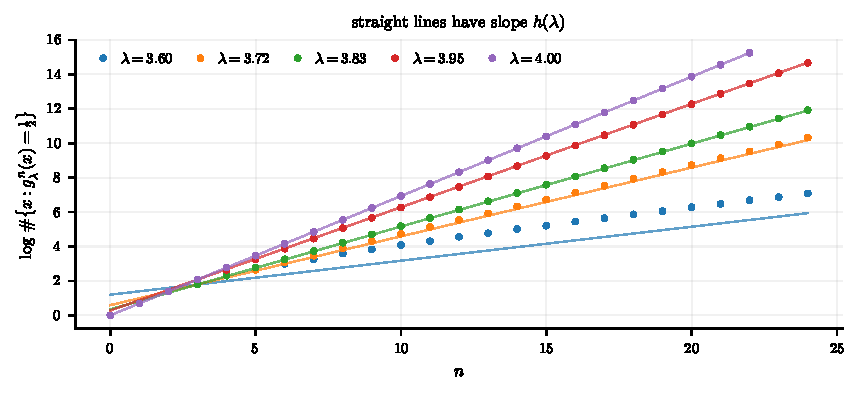
\includegraphics[width=\textwidth]{fig_lapgrowth}
  \caption{The independent check of Theorem~\ref{thm:MS}: the logarithm of the number of
  solutions of $g_\lambda^n(x)=\tfrac12$ against $n$, for five parameters.  The superposed
  straight lines have slope $h(\lambda)$ as computed from the determinant, and are drawn
  through the last point.  The counts approach them as $n$ grows, and the transient --- the
  gap at small $n$ --- is the longer the smaller $h(\lambda)$ is.}
  \label{fig:lapgrowth}
\end{figure}

In the figure the dots approach the lines as $n$ grows, and the approach is the slower
the smaller $h(\lambda)$ is.  At $\lambda=3.60$, where $h=0.197$ is far below $\log2$, the
gap is still $0.34$ nats at $n=8$ and $0.06$ at $n=16$; for $\lambda\ge3.83$ it is below
$0.06$ from $n=2$ onwards, and at $\lambda=4$ the count is exactly $2^n$, so the dots lie on
the line from the start.  The reason is that for small $n$ almost every point has two
preimages and the growth rate starts near $\log2$, relaxing to $h(\lambda)$ only once the
preimage tree is pruned; the smaller $h$ is, the longer that takes.  This is the same
subexponential correction that Table~\ref{tab:laps} measures.  The approach is not always to
a line.  The determinant has $2^k$ zeros of modulus $t_0=e^{-h}$, at $t_0$ times the
$2^k$-th roots of unity, where $k$ is the largest integer with $s^{2^k}\le2$; then
$c_ns^{-n}$, with $c_n$ the number of solutions of $g_\lambda^n(x)=\tfrac12$, carries a
component of period $2^k$ and converges only along residue classes
modulo $2^k$.  For $k=1$ this happens exactly for $\lambda\le3.67857\ldots$, and
$\lambda=3.60$, with $s=1.2183$, is such a parameter --- which is why its dots approach a
band, a component interval of the limit set, rather than a line; the other four have $s\ge1.49$ and $k=0$.  The thresholds
$s^{2^k}=2$ are the band-merging parameters, where the limit set passes from $2^{k+1}$ bands
to $2^k$, and on each band the model map is $f_s^{2^k}$ (companion note).  We
checked the rule at $65$ parameters between $3.5705$ and $3.6985$ without exception.

Figure~\ref{fig:lapsperiod} shows the periodicity on its own.  Plotted as a single sequence,
$\log c_n-h(\lambda)n$ zigzags; split by the residue of $n$ modulo $2^k$ it falls into $2^k$
smooth curves, one for each band.

\begin{figure}
  \centering
  \includegraphics[width=\textwidth]{fig_laps_period}
  \caption{The periodicity of the counts, at two parameters of the companion note.
  $\log c_n-h(\lambda)n$ against $n$, with the points coloured by the residue of $n$ modulo
  $2^k$: (a)~the period-$6$ centre $\lambda=3.6276$, in the two-band range, gives two curves;
  (b)~the period-$12$ centre $\lambda=3.5822$, in the four-band range, gives four.  Each
  colour is smooth while the union zigzags.}
  \label{fig:lapsperiod}
\end{figure}

\subsection{Exact plateaus}

The most conspicuous feature of the graph is the step at $h=\log\tau$, and it is exact.
At $\lambda=3.845$ the computed sign sequence is exactly
$12$-periodic, so $D=P(t)/(1-t^{12})$ with $P$ of degree $11$ and integer coefficients;
$P$ is divisible by $t^2+t-1$, hence $D(1/\tau)=0$ exactly and, since no smaller zero
exists, $h=\log\tau$.  At $\lambda=3.85$, $3.855$ and $3.8565$ a $60$-digit evaluation
gives $|D(1/\tau)|<10^{-60}$.  The step runs from the saddle-node (the parameter where the
period-$3$ cycle is born) $\lambda=1+\sqrt8=3.8284271$ to $\lambda\approx3.8568$, the real extent of the period-$3$
copy of the Mandelbrot set, before $h$ rises again.

The same happens at the other hyperbolic components (windows).  The period-$5$ window, at
$\lambda\approx3.9056$--$3.9068$, has $h=\log s_5=0.543535$ throughout, and the
period-$4$ window, at $\lambda\approx3.9601$--$3.9616$, has $h=\log s_4=0.609378$, where
$s_3=\tau$, $s_4=1.839286755\ldots$ and $s_5=1.722083806\ldots$ satisfy
\[
  s_3^2-s_3-1=0,\qquad s_4^3-s_4^2-s_4-1=0,\qquad s_5^4-s_5^3-s_5^2-s_5+1=0 ;
\]
the equations come from the numerators $t^2+t-1$, $t^3+t^2+t-1$ and
$t^4-t^3-t^2-t+1$ of $D$.  The growth number stays fixed across the cascade.

\begin{figure}
  \centering
  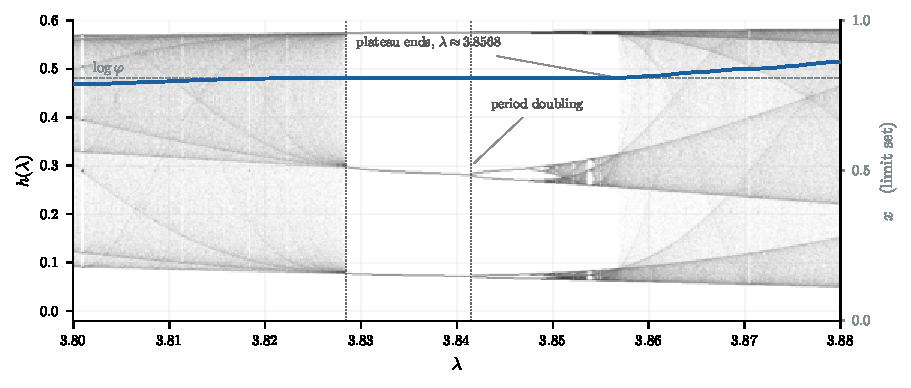
\includegraphics[width=\textwidth]{fig_plateau}
  \caption{Three period-doubling cascades: the period-$3$ window (a), the period-$5$
  window (b) and the period-$4$ window (c), each against its bifurcation diagram.  In
  every panel $h$ is flat across the whole cascade --- at $\log\tau$, $\log s_5$ and
  $\log s_4$ --- and rises only when the window's structure ends.  The horizontal dashed
  line is the plateau level; the dotted lines mark
  the saddle-node and the first period doubling, the dash-dotted line the accumulation of
  the cascade.}
  \label{fig:plateau}
\end{figure}

The plateau in Figure~\ref{fig:plateau} coincides with the period-$3$ window and ends where
the window's structure ends, at $\lambda\approx3.8568$; between the two the entropy does not
move, even though the attracting cycle doubles repeatedly.  Panels~(b) and~(c) show that this
is not special to period $3$.

\section{Concluding remarks}

Two things are proved along the way and one is assumed.  The reduction of the entropy to
the growth rate of lap numbers is a theorem of Misiurewicz and Szlenk, and the identification
of that growth rate with the reciprocal of the smallest zero of the kneading determinant is
a theorem of Milnor and Thurston; the truncation bound \eqref{eq:tail} is elementary and is
what makes the scheme trustworthy, since it converts a series that cannot be summed into a
criterion that can be checked at every parameter.  What is assumed is that the smallest zero
of the truncated determinant is simple, so that the search for a sign change finds it; the
assumption is stated in \S\ref{sec:error} and never failed.  Nothing in the method is
special to the logistic family except the bound $h\le\log2$ that places the zero above
$\tfrac12$: any unimodal family with a computable kneading sequence can be treated the same
way, once the orbit and its signs are supplied.

\begin{thebibliography}{9}\footnotesize\setlength{\itemsep}{1pt}\setlength{\parskip}{0pt}
\bibitem{dMvS} W.~de Melo and S.~van Strien, \emph{One-dimensional dynamics},
Ergebnisse der Mathematik 25, Springer, 1993.
\bibitem{Guck} J.~Guckenheimer, Sensitive dependence on initial conditions for unimodal maps,
\emph{Comm. Math. Phys.} 70 (1979), 133--160.
\bibitem{Sing} D.~Singer, Stable orbits and bifurcation of maps of the interval,
\emph{SIAM J. Appl. Math.} 35 (1978), 260--267.
\bibitem{MT} J.~Milnor and W.~Thurston, On iterated maps of the interval, in
\emph{Dynamical Systems} (College Park, 1986--87), Lecture Notes in Math. 1342,
Springer, 1988, 465--563.
\bibitem{MS} M.~Misiurewicz and W.~Szlenk, Entropy of piecewise monotone mappings,
\emph{Studia Math.} 67 (1980), 45--63.
\bibitem{Tiozzo} G.~Tiozzo, Topological entropy of quadratic polynomials and dimension of
sections of the Mandelbrot set, \emph{Adv. Math.} 273 (2015), 651--715.
\bibitem{Tiozzo2} G.~Tiozzo, Continuity of core entropy of quadratic polynomials,
\emph{Invent. Math.} 203 (2016), 891--921.
\end{thebibliography}

\end{document}
